% !TEX root = main.tex

%%%%%%%%%%%%%%%%%%%%%%%%%%%%%%%%%%%%%%%%%%%%%%%%%%%%%%
\section{実験目的}
%%%%%%%%%%%%%%%%%%%%%%%%%%%%%%%%%%%%%%%%%%%%%%%%%%%%%%
一般に,制御とは「制御対象があらかじめ与えられた望ましい状態に適合するように適当な操作を加えることである」と定義されている.
この操作を完全に装置のみで行うことを自動制御という.自動制御を実現するために必要な素材は,センサ,アクチュエータ,コンピュータである.
本実験では,「倒立振子」と呼ばれる実験装置を制御対象とし,自動制御を実現させるための一連の流れを習得することを目的としている.\\
\quad 1周目の実験では,センサとコンピュータの特性を把握する方法を学ぶ.センサとしては,ロータリエンコーダを用いるが,センサ信号から倒立振子の振子角度や台車位置への変換係数を求める.
また,センサ信号から速度算出を行う際に,ローパスフィルタによる処理の効果を調べる.つぎに,アクチュエータとしてDCモータを用いるが,電力増幅器の極性を調整する.
\quad 2周目の実験では,倒立振子の自動制御を実現するコントローラーを設計するコントローラーを設計する手順を学ぶ.まず,制御対象のモデリングを行う.倒立振子のモデル(微分方程式)は第一原理により得ることができるが,
それに含まれるパラメータの値は未知である.そこで,2次遅れ系の特性に基づいてパラメータの値を決定する.このような操作をパラメータ同期という.つぎに,倒立振子のモデルを状態空間表現で表し,状態フィードバック形式のコントローラを
設計し,倒立振子の安定化を実現する.

\section{倒立振子実験装置の概要}
\subsection{倒立振子実験装置}
倒立振子とは,棒を立てる遊びを自動制御により実現する実験装置である.本実験で用いる倒立振子実験装置のシステム構成図を図2.1に示す.

\quad 図2.1に示すように,倒立振子実験装置では,センサ(ロータリエンコーダ)で検出された振子角度,台車位置を元にコントローラー(パソコン)で
アクチュエータ(DCモータ)に加える電圧を計算し,台車を左右に動かすことにより振子が倒れないように制御することができる.

\begin{figure}[H]
  \centering
  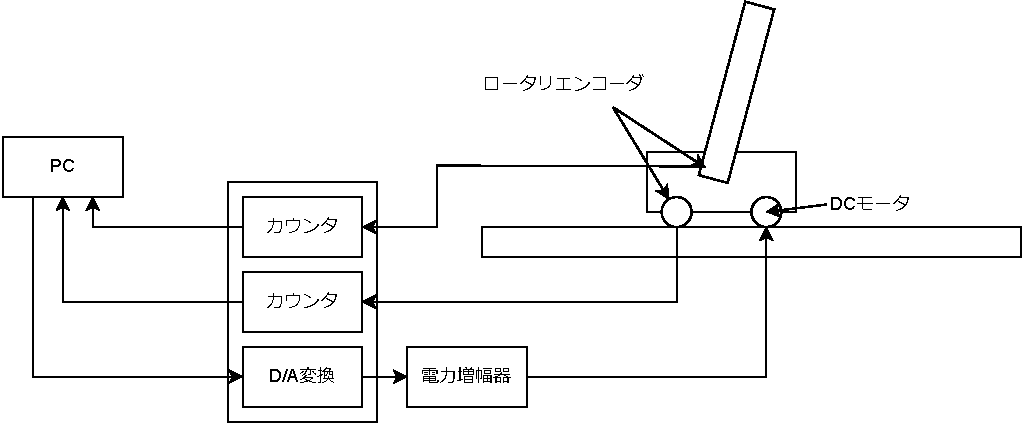
\includegraphics[scale=0.8]{sozai/touritu.pdf}
  \caption{倒立振子実験装置}
\end{figure}

\subsection{ロータリエンコーダとカウンタ}
本実験装置では,大口径のピニオン軸に台車位置検出用,振子軸に振子角度検出用のロータリエンコーダが取り付けられている.いずれもUS digital社製(E2-1024)の光学式/インクリメンタル型
であり,軸が1回転すると1024パルスのA,B信号(ON/OFF信号)が生成される.図2.3に示すようにロータリエンコーダとパソコンはI/OボードQ8-USBのカウンタを
介して接続されている.使用するソフトウェアはQuaRCは,デフォルトでは4逓倍で動作するため,1回転あたり4096カウントとなる

\begin{figure}[H]
  \centering
  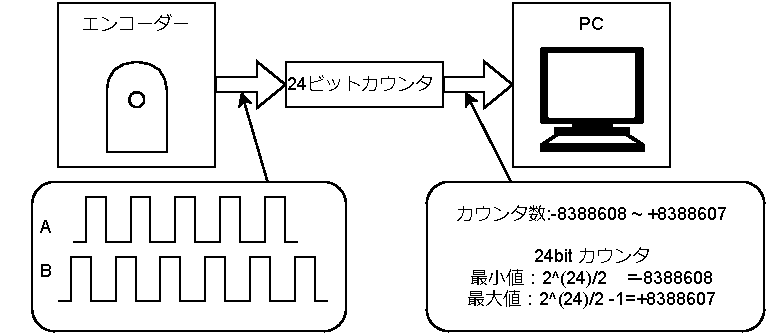
\includegraphics[scale=1]{sozai/encordertokaunnta.pdf}
  \caption{エンコーダーとカウンタ}
\end{figure}

\subsection{DCモータとD/A変換}
本実験装置では,台車を左右に動かすために,少口径のピニオン軸にDCモータが取り付けられている.
パソコンからD/A変換を介して出力された指令電圧は小電力であるため,このままではDCモータを高速回転させることはできない.そこで図2.3に示す
リニア方式の電力増幅器を介して,指令電圧をDCモータに加える.

\begin{figure}[H]
  \centering
  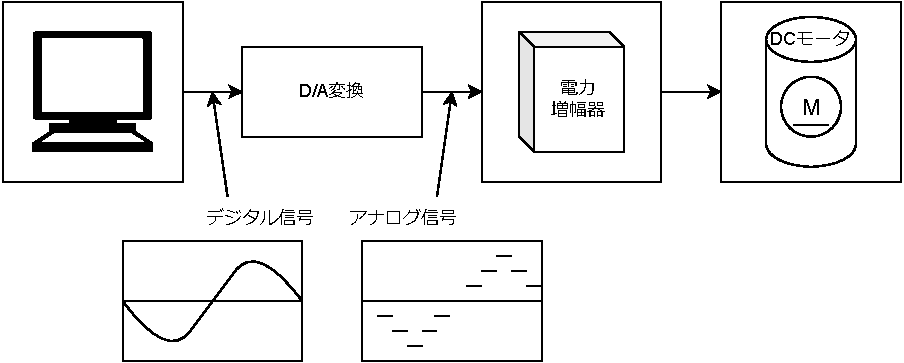
\includegraphics[scale=1]{sozai/DCmotaADhenkan.pdf}
  \caption{エンコーダーとカウンタ}
\end{figure}

\subsection{速度算出}

ロータリエンコーダから台車位置 \( z(t) \) [m] を検出することができれば,h が微小であるとき,近似的に速度を

\begin{equation}
  \dot{z}(t) = \lim_{h \to 0} \frac{z(t) - z(t-h)}{h} \quad [m/s] \backsimeq  \frac{z(t) - z(t-h)}{h} \quad [m/s]
\end{equation}

により算出することができる.ここで,h [s] をセンシングのサンプリング周期とすると,\ t = 0, 1, 2, ... \,であるので,\ k \  番目のサンプリング時刻での位置を \( z[k] = z(kh) \) と記述することにより,(2.1) 式は

\begin{equation}
  \dot{z}[k] = \frac{z[k] - z[k-1]}{h} \quad [m/s]
\end{equation}

のように差分式で記述できる.(2.2) 式を後退差分近似 (オイラー近似) という.
ロータリエンコーダはデジタルセンサのため,接触ノイズを考えなくて良いが,検出される値は離散値であり,量子化誤差が発生する.
この量子化誤差のため,(2.2) 式よりも算出される速度にには高周波成分が含まれてしまう(チャタリング).そこで,ローパスフィルターを利用し

\begin{equation}
  \hat{z_f}[k] = G_f(s) \dot{z}(t), \quad G_f(s) = \frac{1}{1 + T_f s} \quad (T_f > 0)
\end{equation}

のようにしてチャタリングを除去する(図 2.8).

\begin{figure}[H]
  \centering
  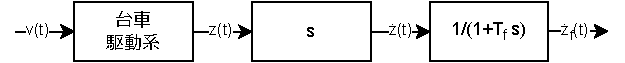
\includegraphics[scale=1]{sozai/ro-pasufiruta.pdf}
  \caption{ローパスフィルタ}
\end{figure}

\newpage

\section{実験1}

\subsection{実験装置のセッティング}
\noindent
以下のことに注意する.

\begin{itemize}
  \item モータを動かす必要のある実験を行うときのみ,Universal Power Module の電源をONにすること.
  \item モータを動かす実験が終了した後は必ず Universal Power Module の電源をOFFにすること.
  \item モータを動かす実験を行うときには必ず1人が Universal Power Module のスイッチに触れておき, 暴走した場合にはただちに電源をOFFにすること,
\end{itemize}

\subsection{実験1-1: 振子角度とロータリエンコーダの動作}

\subsubsection{実験方法}
\noindent
ここでは,図3.2に示す振子の角度変位\(\theta (t)\)[rad]とロータリエンコーダのカウント数の関係を調査する.

\paragraph{実験1-1a}
\begin{enumerate}
  \item \quad 振子側のロータリエンコーダとカウンタの動作確認をする別紙「補足事項:QusRCの使用方法」を参考にして,
        図A.1のSimulinkモデル"pend\_count.slx"を作成し,ディレクトリ
        [D:\textbackslash experiment\_5S\textbackslash group01\textbackslash pend\_encoder]に保存する.
        また,ビルドしてエラーがないことを確認した後,
        
        \begin{tcolorbox}[colback=gray!5!white,colframe=gray!75!black]
          \begin{lstlisting}
        >> print -dpdf = pend_count.pdf
        >> load('pend_count.temp')
        \end{lstlisting}
        \end{tcolorbox}
        
        と入力してpdfファイル,bmpファイルを生成する.
        
  \item \quad Universal Power Moduleの電源がOFF担っていることを確認する.
        振子を取り付けて振子がぶら下げた状態に静止させ, Simulinkモデルを実行する.
        振子がぶら下がった状態から時計回り(あるいは反時計回り)に振子を手で回転させたときのロータリエンコーダのカウント数を
        Displayにより観測された値を表にまとめる. 表 3.1に記入 \\
        \quad 観測を終えたら,Simulink モデルの実行を終了させる.
        
  \item \quad 表 3.1の関係から,1カウントあたりの振子の角度変位  \(\alpha \) [rad/カウント] (時計回りを正とする)
        を求める.
        
        \begin{figure}[h]
          \centering
          \begin{minipage}{0.45\textwidth}
            \centering
            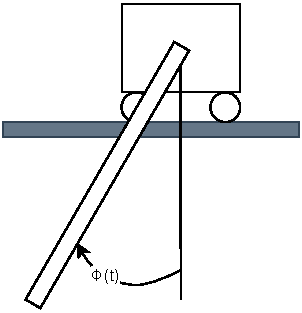
\includegraphics[scale=0.9]{sozai/shinnshinokakudohenni.pdf}
            \caption{振子の角度変位}
          \end{minipage}
          \hfill
          \begin{minipage}{0.45\textwidth}
            \centering
            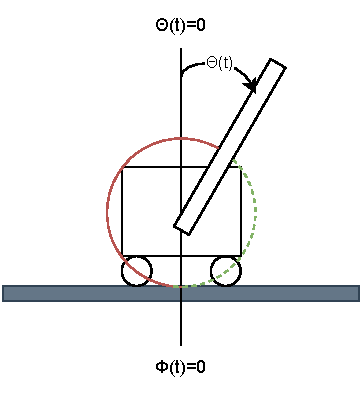
\includegraphics[scale=0.75]{sozai/theta_relation.pdf}
            \caption{φ(t)とθ(t)との関係}
          \end{minipage}
        \end{figure}
        
\end{enumerate}

\paragraph{実験1-1b}
\begin{enumerate}
  \item 図 A.2のSimulinkモデル "pend\_count2.slx" を作成し,
        振子を時計回りに1 回転したとき測定値が2\(\pi\)[rad](360[deg]) 
        となるようにする("pend\_count2.slx" は [D:\textbackslash experiment\_5S\textbackslash group01\textbackslash pend\textbackslash pend\_encoder]に保存すること). 
        ただし, Gain (count to rad) は 実験 1-1 で求めた値 
        (ただし, "1000/pi" などのように計算式をそのまま入力する), 
        Gain (rad to deg) は [rad] から [deg] への
        変換係数 "180/pi" を設定する. 
        また, "pend\_count2.slx" をビルドしてエラーがないことを確認した
        後, "pend\_count2.pdf", "pend\_count2.bmp" という名前の 
        pdf ファイル, bmp ファイルを生成する
        
  \item 実験を開始し, Display (count), Display (rad), Display (deg) により運動を知た値を表にまとめる.
        観測を終えたら, Simulink モデルの実行を終了させる.
\end{enumerate}

\paragraph{実験 1-1c}

\begin{enumerate}
  \item 振子がぶら下がった状態を基準とした角度変位 \(\theta(t)\) と倒立状態を基準とした角度変位 \(\phi(t)\) との関係は
        \begin{equation}
          \theta(t) = 
          \begin{cases}
            \phi(t) - \pi & (\phi(t) \geq 0: \text{時計回りに回転}) \\
            \phi(t) + \pi & (\phi(t) < 0: \text{反時計回りに回転}) 
          \end{cases}
        \end{equation}
        である(図 3.2 参照).ただし,\(\phi(t)\),\(\theta(t)\) ともに時計回りを正とする.
        振子がぶら下がった状態から時計回り(あるいは反時計回り)
        に回転させたとき,振子の倒立点で角度変位が 0 [rad]
        (0 [deg]) となるように図 A.2 の Simulink モデルを
        修正し,D:\textbackslash experiment\_5S\textbackslash group01\textbackslash pend\textbackslash pend\_encoder 
        に "pend\_count3.slx" という名前で保存する.
        また,"pend\_count3.slx" をビルドしてエラーがないことを
        確認した後,"pend\_count3.pdf","pend\_count3.bmp" 
        という名前の pdf ファイル,bmp ファイルを生成する
        
  \item 振子がぶら下がった状態で静止していることを確認した後,
        実験を開始し,Display (deg) により振子の角度 \(\theta(t)\) [deg]
        を観測し,その値を表にまとめる.
        観測を終えたら,Simulinkモデルの実行を終了させる.
        なお実験では,手で振子を時計回り(あるいは反時計回り)
        に回転させたとき,振子の倒立状態でのθ(t)が0[deg]となっていることを
        確認した後,振子を右側に水平とするとθ(t)が90[deg],
        振子を左側に水平とするとθ(t)が-90[deg]となっていることを確認する.
\end{enumerate}

\subsubsection{実験結果}

\paragraph{実験 1-1a}
図 A.1 の Simulink モデルを実行したときに得られた結果を表 に示す.また,1カウントあたりの角度変位は

\[
  \alpha = \frac{2 \pi}{4096}\thickapprox 1.534\times 10^{-3}{\large\textbf{}[rad/カウント]}
\]

である(計算式も記入すること).

\begin{table}[h]
  \centering
  \caption{ロータリエンコーダとカウンタの動作確認(振子)}
  \label{tab:rotation}
  \begin{tabular}{|c|c|}
    \hline
    回転の方向                       & 測定値 [カウント] \\
    \hline
    時計回りに1回転(+ 360 [deg])   & -4096             \\
    反時計回りに1回転(- 360 [deg]) & 4096              \\
    \hline
  \end{tabular}
\end{table}
\paragraph{実験 1-1b}
図A.2のSimulinkモデルを実行したときに得られた結果を表3.2に示す.

\begin{table}[h]
  \centering
  \caption{"pend\_count2.slx" の動作確認(カウント数から角度変位への変換)}
  \label{tab:pend_count2}
  \begin{tabular}{|c|c|c|c|}
    \hline
    回転の方向                      & 測定値 [カウント] & 測定値 [rad] & 測定値 [deg] \\
    \hline
    時計回りに1回転(+360 [deg])   & -4096             & 6.283        & 360          \\
    反時計回りに1回転(-360 [deg]) & 4096              & -6.283       & -360         \\
    \hline
  \end{tabular}
\end{table}

\paragraph{実験 1-1c}
Simulink モデルを実行したときに得られた結果を表 \ref{tab:pend_count3} に示す.
なお,角度はおおよそその値で良く,0, 90, -90 のいずれかを記入すること.

\begin{table}[h]
  \centering
  \caption{"pend\_count3.slx" の動作確認(倒立点を基準とした角度 $\theta(t)$)}
  \label{tab:pend_count3}
  \begin{tabular}{|c|c|c|c|c|c|}
    \hline
    回転方向 & 振子の状態   & 測定値 [deg] & 回転方向   & 振子の状態   & 測定値 [deg] \\
    \hline
    時計回り & 倒立(真上) & 0            & 反時計回り & 倒立(真上) & 0            \\
             & 右水平       & 90           &            & 右水平       & 90           \\
             & 左水平       & -90          &            & 左水平       & -90          \\
    \hline
  \end{tabular}
\end{table}


\subsubsection{実験考察}
\paragraph{考察事項1}
エンコーダーは,回転や移動を検知するためにスリットと呼ばれる目盛りが設けられている.
「4096」という値は,エンコーダーの分解能を示す数値で,1回転あたり4096のパルスが
検出されることを意味している.
逓倍とは,エンコーダーのパルス信号をさらに細かく分割する技術のことであり,
4逓倍の場合は1つのスリットに対して4つのパルス信号を生成することげできる.
エンコーダーのスリット数が1024である場合,基本的な分解能は1回転あたり1024パルスであるが,
この信号を4逓倍すると
\( 1024\times 4=4096 \) となる.
このように,スリット数1024に対して4逓倍を行うことで,
実際には1回転あたり4096パルスの分解能が得られる.

\paragraph{考察事項2}
ロータリエンコーダ自体は角度を出力するものではなくパルスを出力している.
つまり受取側,例えばマイコンやi/oボードなどがパルスを受取計算する.
そのため基準点は処理側のリセットを用いている.


\paragraph{考察事項3}
ポテンショメータでは倒立振子の角度を計測するのには向いていない.
理由として摩擦が挙げられる.ロータリエンコーダの場合,回転時にほとんど摩擦が発生しないが,ポテンショメータの場合
摩擦が発生している.摩擦が発生すると倒立振子の棒に力がかかってしまう.

\paragraph{考察事項4}
基準からどちらに回転したかによって式を変える必要がある.
そのためこのSimulinkモデルでは,Switchを使用し角度変位からを加減するかを判断している.
Switchに入力する際に\( + \)であるとき,\( \pi \)を引き,\( - \)であるとき,\( \pi \)を足している.

\begin{figure}[h]
  \centering
  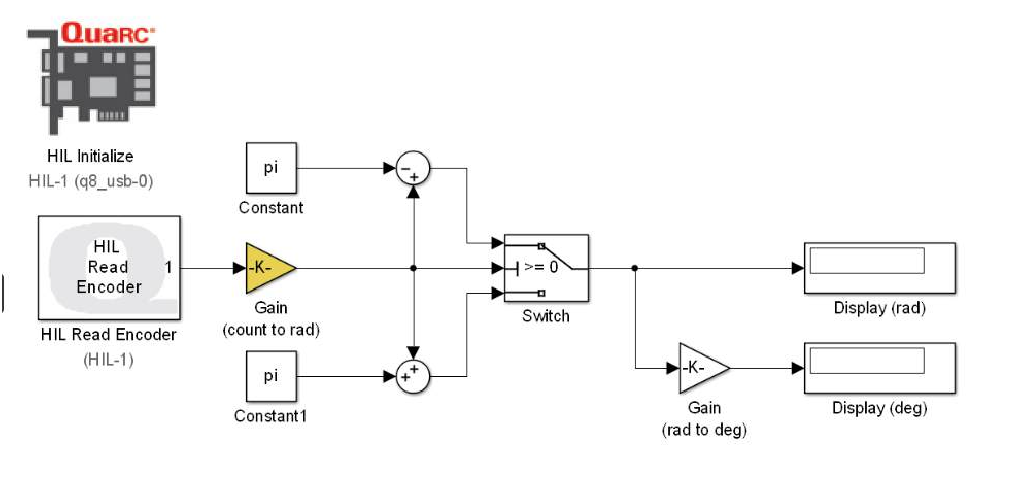
\includegraphics[scale=0.9]{sozai/pendcount3.pdf}
  \caption{シミュリンクモデル}
\end{figure}


\subsection{実験1-2: 台車位置とロータリエンコーダの動作}

\subsubsection{実験方法}
ここでは,図 3.3 に示す台車の位置変位 \( z(t) \) [m] とロータリエンコーダのカウント数の関係を調べる.

\begin{figure}[h]
  \centering
  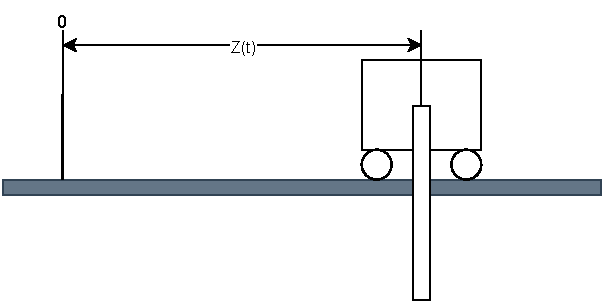
\includegraphics[scale=1]{sozai/daisyanoichihenni.pdf}
  \caption{台車の位置変位 \( z(t) \)}
\end{figure}


\paragraph{実験1-2a}
\begin{enumerate}
  \item 台車側のロータリエンコーダとカウンタの動作確認をする図 A.3 の Simulink モデル
        "cart\_count.slx" を作成し,D:\textbackslash experiment\_5S\textbackslash group01\textbackslash cart\_encoder に保存する.
        また,ビルドでエラーがないことを確認した後,"cart\_count.pdf", "cart\_count.bmp" 
        という名前の pdf ファイル,bmp ファイルを生成し,pdf ファイルはデスクトップ上の 
        "bcpdfcrop-multi.bat" により余白を取り除く.
        
  \item Universal Power Module の電源がOFFになっていることを確認し,Simulink モデルの実行を開始する.台車を手で右方向(あるいは左方向)に 0.8 [m] 移動させたときのロータリエンコーダのカウント数を Display により観測する.これを 4 回,繰り返す.表にまとめる.表 3.4 に記入し,観測を終えたら,Simulink モデルの実行を終了させる.
        
  \item 図 3.4 の結果を利用し,1 カウントあたりの台車の位置変位 \( \beta \) [m/カウント] を求める.
\end{enumerate}

\paragraph{実験 1-2b}
\begin{enumerate}
  \item 図 A.4 の Simulink モデル "cart\_count2.slx" を作成し,台車を右方向に 1 [m] 移動させたときに測定値が
        +1 [m] となるようにする("cart\_count2.slx" は D:D:\textbackslash experiment\_5S\textbackslash group01\textbackslash pend\textbackslash pend\_encoder に保存すること).
        ただし,Gain は実験 1-2a で求めた \(\beta\) の値に設定する.また,"cart\_count2.slx" を
        ビルドしてエラーがないことを確認し,"cart\_count2.pdf","cart\_count2.bmp" という名前の 
        pdf ファイル,bmp ファイルを生成し,pdf ファイルはデスクトップ上の "bcpdfcrop-multi.bat" により
        余白を取り除く.\\
        
  \item Simulink モデルの実行を開始し,Display (meter), Display (count) により観測された値を
        表にまとめる.表 3.5 に記入し,観測を終えたら,Simulink モデルの実行を終了させる.
        
\end{enumerate}


\subsubsection{実験結果}

\paragraph{実験 1-2a}
図 A.3 の Simulink モデルを実行したときに得られた結果を表 \ref{tab:exp_1_2a} に示す.これより,1カウントあたりの位置変位は

\[
  \beta =  \frac{0.8}{35277.75}\thickapprox 2.268\times 10^{-5}{\large\textbf{}[m/カウント]}
\]

である.

\begin{table}[h]
  \centering
  \caption{ロータリエンコーダとカウンタの動作確認(台車)}
  \label{tab:exp_1_2a}
  \begin{tabular}{|c|c|c|c|}
    \hline
    \multicolumn{2}{|c|}{(a) 右方向に 0.8 [m] (+0.8 [m])移動} & \multicolumn{2}{|c|}{(b) 左方向に 0.8 [m] (-0.8 [m])移動}                             \\
    \hline
                                                                & 測定値 [カウント]                                           &       & 測定値 [カウント] \\
    \hline
    1回目                                                       & 35348                                                       & 1回目 & -35273            \\
    \hline
    2回目                                                       & 35345                                                       & 2回目 & -35157            \\
    \hline
    3回目                                                       & 35277                                                       & 3回目 & -35273            \\
    \hline
    4回目                                                       & 35276                                                       & 4回目 & -35273            \\
    \hline
  \end{tabular}
\end{table}

\paragraph{実験 1-2b}

図 A.4 の Simulink モデルを実行したときに得られた結果を表 \ref{tab:exp_1_2b} に示す.

\begin{table}[h]
  \centering
  \caption{"cart\_count2.slx" の動作確認(カウント数から位置変位への変換)}
  \label{tab:exp_1_2b}
  \begin{tabular}{|c|c|c|}
    \hline
    移動方向・距離                    & 測定値 [カウント] & 測定値 [m] \\
    \hline
    右方向に 0.5 [m] (+0.5 [m])移動 & 22034             & 0.4997     \\
    \hline
    左方向に 0.5 [m] (-0.5 [m])移動 & -21808            & -0.4945    \\
    \hline
  \end{tabular}
\end{table}

\subsubsection{実験考察}
表3.4より,0.8[m]動かしたときに平均35277.75カウントを行った.
これにより\( \beta =  \frac{0.8}{35277.75}\thickapprox 2.268\times 10^{-5}\)となり求めることができた.
台車を0.1[m]ではなく0.8[m]動かした理由としては全体の誤差を少なくするためである.
手動で回しているため,停止時に誤差が含まれる.そのときに発生する誤差が全体を占める割合を小さくするために
測定値を大きくさせた.
位置検出の精度に関しては計算により最低\(2.268\times 10^{-5}\)[m]ピッチで位置推定できる.
また,他に \(\beta\) を求める方法としてラックピニオンのモジュールなどの歯車の数を活用できる.

\subsection{実験1-3: DCモータとD/A変換の動作}

\subsubsection{実験方法}
\begin{enumerate}
  \item 図 A.5 の Simulink モデル "da\_conv.slx" を作成し,
        D:\textbackslash experiment\_5S\textbackslash group01\textbackslash da に
        保存する.ただし,終了時間を 1 秒に設定する(\textbf{絶対に忘れないこと!!}).また,
        ビルドしてエラーがないことを確認した後,"da\_conv.pdf","da\_conv.bmp" という名前の
        pdf ファイル,bmp ファイルを生成し,pdf ファイルはデスクトップ上の 
        "bcpdfcrop-multi.bat" により余白を取り除く.
        
  \item 台車をレールの中央付近に配置する.Universal Power Module の電源を ON にした後,
        Simulink モデルの実行を開始する.D/A 変換を介して DC モータに一定の電圧が加わり,
        台車がほぼ一定速度で移動する.正の電圧 +1 [V],負の電圧 -1 [V] を加えたときに台車が
        左右どちらの向きに移動するのかを観察し,表 3.6 に記入する.
        
\end{enumerate}

\subsubsection{実験結果}
図 A.5 の Simulink モデルを実行したときの実験結果を表 3.6 に示す.

\begin{table}[h]
  \centering
  \caption{指令電圧と台車の移動方向}
  \label{tab:command_voltage_direction}
  \begin{tabular}{|c|c|}
    \hline
    指令電圧 [V] & 移動方向 \\
    \hline
    +1           & 右       \\
    \hline
    -1           & 左       \\
    \hline
  \end{tabular}
\end{table}

\subsubsection{実験考察}
\paragraph{考察事項1}
+1[V]の指令を与えたときに台車が左方向に移動する場合,このままでは極性が逆である.このように極性を間違えた状態でフィードバック制御
を行うと発散してしまう.
理由として離れようとして出力が上がるとさらに差が大きくなり,より出力を上げようとしてしまう.
このように差が,収束するどころか大きくなり続けてしまう.

\paragraph{考察事項2}
極性を反転させる方法として,ハードウェア側の調整だとDCモータに接続されている線を反転させるかエンコーダーに接続された信号線を反転させる方法が挙げられる.
ソフトウェア側での調整は出力する電圧の符号を反転するか,エンコーダーの角度の符号を反転するなどが挙げられる.


\subsection{実験1-4: 台車の速度算出}

\subsubsection{実験方法}
\begin{enumerate}
  \item カレントディレクトリを D:\textbackslash experiment\_5S\textbackslash group01\textbackslash da\_encoder とし,配布する Simulink モデル "da\_conv\_count.slx"(図 A.6)を開く.そして,Simulink ブロックを
        \begin{itemize}
          \item Gain (polarity): ゲインに "1" もしくは "-1" を入力(3.4 節を参照)
          \item Gain (count to meter): ゲインを1カウントあたりの台車位置変位 Δl に変更
                (3.3 節を参照)
        \end{itemize}
        
        と設定し,書き保存する.また,ビルドしてエラーがないことを確認した後,
        "da\_conv\_count.pdf","da\_conv\_count.bmp" という名前の 
        pdf ファイル,bmp ファイルを生成し,pdf ファイルはデスクトップ上の 
        "bcpdfcrop-multi.bat" により余白を取り除く.
        
  \item 台車をレールの中央付近に配置する.Universal Power Module の電源を ON にした後,
        Simulink モデルの実行を開始する.D/A 変換を介してDCモータに一定の電圧 
        u(t) = 1 [V] が加わり,台車が右方向に移動する.実行終了後,
        
        \begin{tcolorbox}[colback=gray!5!white,colframe=gray!75!black]
          \begin{lstlisting}
  >> save filter_data = t dz dzf1 dzf2 dzf3
  \end{lstlisting}
        \end{tcolorbox}
        
        と入力し,実験デーsタを "filter\_data.mat" という名前の mat ファイルに保存する.
        
  \item 配布する M ファイル "plot\_filter.m" を実行することによってグラフを描く.
\end{enumerate}

\subsubsection{実験結果}

\begin{figure}[h]
  \centering
  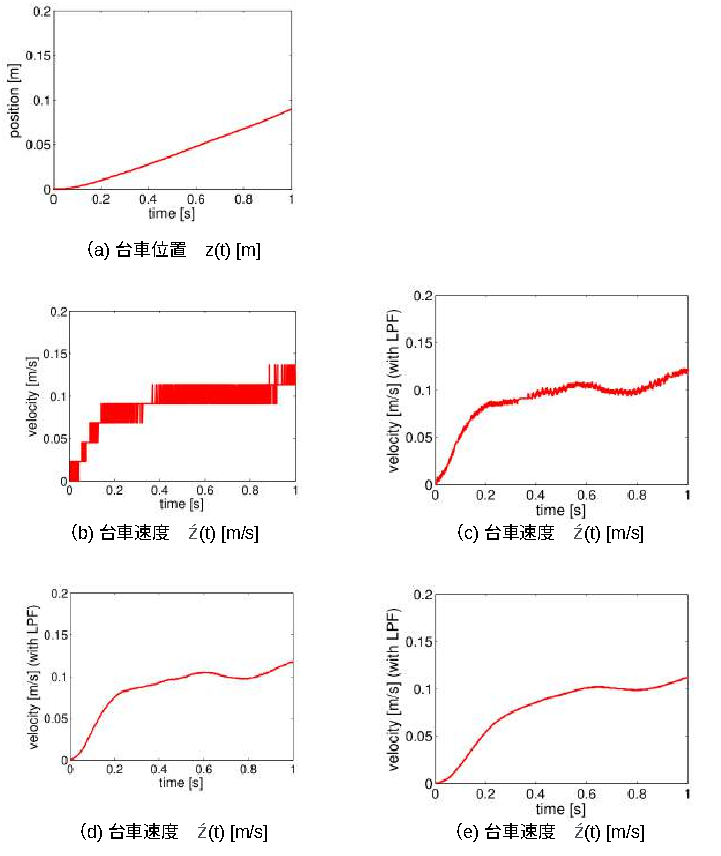
\includegraphics[scale=1]{sozai/3.pdf}
  \caption{台車の位置と速度}
\end{figure}


\subsubsection{実験考察}
図3.5より速度が一定でないことがわかる. 理由として,モーターの加速時間と摩擦が関係していると考えられる.
モータ始動時に電流が流れるが,一定速度になるまで電流を流してから少し時間がかかる.また,静止摩擦の影響も考えられる.
停止している物体には静止摩擦が働くが,動き出すと動摩擦に変わる.そのため,動き出しで抵抗が小さくなる.
量子化は,連続的なアナログ信号を離散的なデジタル値に変換することができるが,図3.5(b)のようにチャタリングが
発生している.これは微小な変動が量子化レベルの間で発生すると,デジタルデータが不安定に振動し,
チャタリングが発生すると考えられる.そこで対策としてローパスフィルターの適応が挙げられる.
ローパスフィルターを適用して,高周波成分やノイズを除去することで,チャタリングを軽減することができる.
ローパスフィルターの時定数 \(\mathcal{T}\)はが大きいと,フィルターの応答が遅くなる.
この場合,高周波成分がより効果的に減衰され,チャタリングのような高速な変動が大幅に抑えることができる.


\begin{figure}[h]
  \centering
  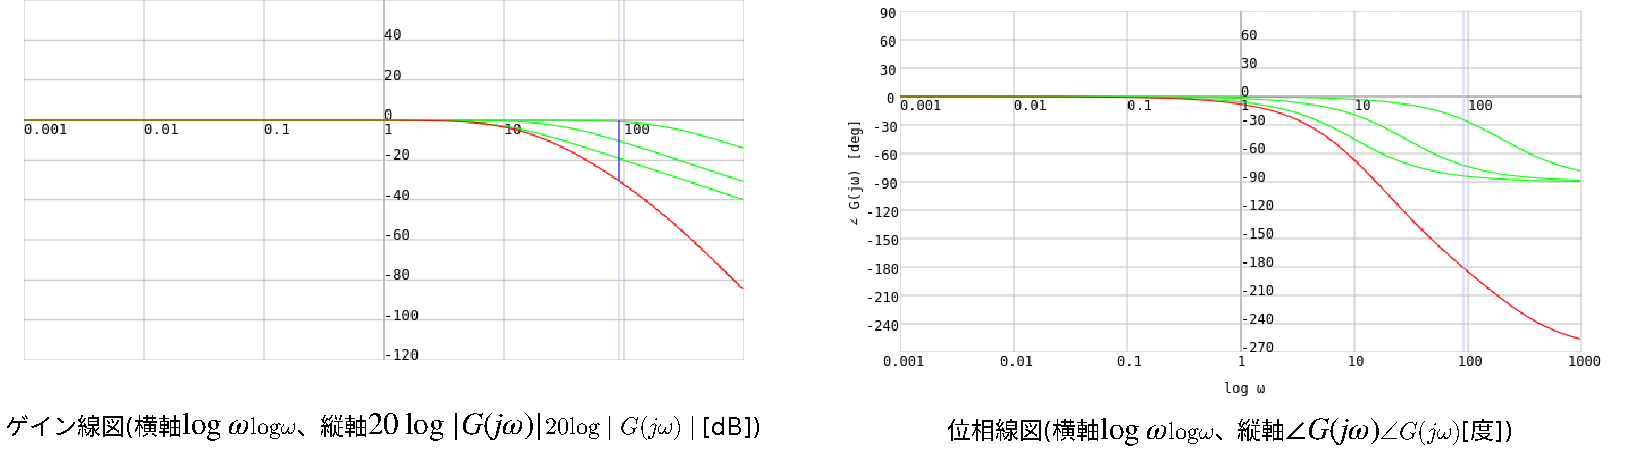
\includegraphics[scale=0.65]{sozai/4.pdf}
  \caption{ボード線図}
\end{figure}
